\section{Cycles in the Energy Model} \label{cycles}

In this section, we show that two agents suffice to obtain a $1$-competitive algorithm for the exploration
of cycles in the energy model. For this we modify the \textit{ALE Algorithm} by Higashikawa et al.\ \cite{Higashikawa2012}. We first show 
that the \textit{ALE Algorithm} has a competitive ratio greater than $1$ in the energy model. After that we construct a modified
algorithm and prove that it reaches $1$-competitiveness in the energy model.

\subsection{ALE is $1.5$-competitive in the energy model}


\begin{theorem}[The \textit{ALE} algorithm and the energy model]\label{AleLowerTad}
    The \textit{ALE} algorithm has a competitive ratio of $1.5$ in the energy model on cycles.
\end{theorem}


\begin{figure}[H]
    \begin{center}
    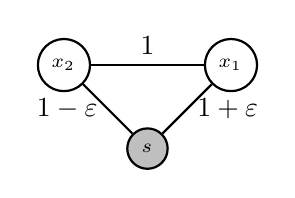
\begin{tikzpicture}[node distance={15mm}, thick, main/.style = {draw, circle}, scale=0.5] 
        \node[main, fill=gray!50, minimum size=0.5cm] (2) {$_{s}$ }; 
        \node[main, minimum size=0.5cm] (1) [above left of = 2] {$_{x_2}$ }; 
        \node[main, minimum size=0.5cm] (3) [above right of = 2] {$_{x_1}$ }; 
        \draw (1) to node[left] {$1-\varepsilon$} (2);
        \draw (2) to node[right] {$1+\varepsilon$} (3);
        \draw (3) to node[above] {$1$} (1);
    \end{tikzpicture} 
    \end{center}
    \caption[ALE is not $1$-competitive]{Since $(s,x_1)$ is the longest edge, one agent moves clockwise from $s$ to $x_1$.}\label{ale}
\end{figure}

\begin{proof}
    Let $0 < \varepsilon < 0.5$. Consider the graph shown in Figure \ref{ale}. Since $(s,x_1)$ is the longest edge in the graph, one agent explores the graph clockwise from $s$ to $x_1$. After the agent
    reaches $x_1$ the shortest path to $s$ is the edge $(x_1, s)$, leading to a cost of $3$. An optimal strategy would have sent both agents from $s$ to $x_1$ 
    and $x_2$ respectively, leading to an exploration cost of $2(1+\varepsilon)$. The overhead of ALE in this case is $\frac{3}{2(1+\varepsilon)}$, leading to a competitive ratio of
    $1.5$ for arbitrary small $\varepsilon$.
\end{proof}

\subsection{The AMP Algorithm}

To construct a $1$-competitive algorithm for the energy model we make use of an observation made by Higashikawa et al.\ concerning the optimal offline exploration 
of a cycle \cite{Higashikawa2012}. Given a cycle graph $C=(V,E)$, a starting node $s \in V$, and the midpoint of the cycle $m$. Then there are two cases:

\begin{enumerate}
    \item $m$ falls onto a node $v_{mid} \in V$ 
    \item $m$ falls onto an edge $e_{mid} = (v_\ell, v_s) \in E$ 
\end{enumerate}

In case 1 the optimal offline strategy sends two agents clockwise and counterclockwise to $v_{mid}$ and back, leading to an exploration time of exactly $L$. In case 2 the agents
are sent to $v_\ell$ and $v_s$ and back, while the edge $e_{mid}$ is not traversed by any agent. The following algorithm sends the agents around the cycle in opposite directions,
with only one moving agent at a time, like the \textit{ALE Algorithm} does, but instead of choosing the locally cheaper edge in each step, the edge which minimizes the distance
traversed by any agent up to that point is chosen. We show that with this change the agents traverse exactly the same paths as the offline optimal strategy, leading to a competitive ratio
of $1$ for the energy model while still achieving the optimal competitive ratio of $1.5$ for the time model.


    \begin{algorithm}[H]
        \caption{AMP (Avoid Midpoint)}\label{alg:cap}
        \begin{algorithmic}
        \small
        \Require A unknown cycle graph $G=(V,E)$, Two agents $a_1, a_2$, a starting node $s \in V$
        \State $d(a_1) \gets 0; d(a_2) \gets 0$ \Comment{Agents track their already traversed distance}
        \State $Exp \gets \{s\}$ \Comment{Keep track of already explored vertices}
        \State Let $n(a_1)$ and $n(a_2)$ describe the next nodes seen by the agents
        \State Assign the two neighbors of $s$ randomly to $n(a_1)$ and $n(a_2)$
        \While{$n(a_1) \not\in Exp \lor n(a_2) \not\in Exp$} \Comment{While graph is not explored}
        \If{$d(a_1) + l(n(a_1)) < d(a_2) + l(n(a_2))$}  
            \State $a_1$ traverses edge to $n(a_1)$ 
            \State $Exp \gets Exp \cup \{n(a_1)\}$
            \State $d(a_1) \gets d(a_1) + l(n(a_1))$
            \State $n(a_1) \gets$ next revealed node
        \Else 
            \State $a_2$ traverses edge to $n(a_2)$
            \State $Exp \gets Exp \cup \{n(a_2)\}$
            \State $d(a_2) \gets d(a_2) + l(n(a_2))$
            \State $n(a_2) \gets$ next revealed node
        \EndIf
        \EndWhile
        \State $a_1$ and $a_2$ return to $s$ using their shortest paths.
        \end{algorithmic}
        \end{algorithm}

\begin{theorem}[Cycles in the Energy Model]\label{ampCycles}
    For the energy model, the \textit{AMP (Avoid Midpoint)} Algorithm \ref{alg:cap} explores a cycle with
    a competitive ratio of $1$. For the time model the algorithm explores a cycle with
    a competitive ratio of $1.5$.
\end{theorem}


\begin{proof}
    We can prove the $1$-competitiveness of the \textit{AMP algorithm} for the energy model, by showing that
    the agents only traverse the cycle to $v_s$ and $v_\ell$ (or $v_{mid}$) before returning, and never traverse the edge $e_{mid}$. We then use this result to prove
    the $1.5$-competitive ratio for the time model.

    \paragraph*{Energy Model} If both agents reach $v_{mid}$ at the same time, all nodes have been visited and both agents have traversed a distance of $L/2$ before and $L$ after backtracking, which matches 
    the result of the optimal offline strategy.\\
     If an agent $a_1$ reaches $v_{mid}$ first, having traversed a distance $d_1 = L/2$, the other agent $a_2$ must have traversed a distance $d_2 < d_1$. Thus, $a_2$ moves to $v_{mid}$ without stopping.
     Then both agents have traversed a distance of $L/2$ when all nodes have been visited and $L$ after backtracking.\\
    Assume w.l.o.g an agent $a_1$ is currently located on $v_s$ after having traversed distance $d_s$ and has not yet traversed $e_{mid}$, while the other agent $a_2$ has not reached $v_\ell$ yet.
    Since $d_\ell < L/2 < d_s + l(e_{mid})$ the agent $a_2$ traverses to $v_\ell$ without stopping. At this point all nodes have been visited and the agents backtrack, having taken the same paths
    as they would have in an optimal offline exploration.

    \paragraph*{Time Model} Recall that an optimal strategy takes time $2d_\ell$. In the AMP algorithm, the agents traverse the distances $d_s$ and $d_\ell$. 
    Since only one agent is traversing an edge at a time until all nodes have been visited, the maximum 
    time needed to visit all nodes is $d_s + d_\ell \leq 2d_\ell$. After backtracking to $s$ the full exploration time is at most $3d_\ell$, leading to a competitive ratio of $1.5$.
\end{proof}